\chapter{Benchmark}
gfortran installieren:
\begin{lstlisting}[style=Bash]
$ sudo apt-get install gfortran sysfsutils cpufrequtils libmpich2-dev
\end{lstlisting}
Für ATLAS muss Cpu Throttling deaktiviert sein.\\
Cpu Throttling deaktivieren: 
\begin{lstlisting}[style=Bash]
$ sudo cpufreq-set -g performance
\end{lstlisting}
ATLAS installieren:
\begin{lstlisting}[style=Bash]
$ ./configure && make
\end{lstlisting}
hpcc downloaden:
\begin{lstlisting}[style=Bash]
$ wget http://icl.cs.utk.edu/projectsfiles/hpcc/download/ \
	hpcc-1.4.3.tar.gz
$ tar -xf hpcc-1.4.3.tar.gz
\end{lstlisting}
Make Konfiguration in hpl als Make.CoreI2 ablegen:
\begin{lstlisting}[style=Bash]
...
\end{lstlisting}
Kompilieren:
\begin{lstlisting}[style=Bash]
$ make arch=CoreI2
\end{lstlisting}
Ausführen:
\begin{lstlisting}[style=Bash]
$ /shared/tools/openmpi/1.8.4/bin/mpirun -n 6 -hostfile \
	/shared/mpi_hosts ./hpcc
\end{lstlisting}
Die theoretische Peak Performance liegt bei ca 1.8GHz*2(Cores)*3(Nodes)*4(FLOPs per cycle) = 43.2 Gflops.
Die 4 FLOPs ergeben sich durch die SSE Extension. SSE ist eine SIMD (Single Instruction Multiple Data) Erweiterung.
Der unoptimierte Durchlauf erreicht 33.41 Gflops. Es werden 77\% der theoretischen Peak Performance erreicht.
Gründe hierfür sind unter anderem die langsame Kommunikation zwischen den CPUs, langsame Speicheranbindung und nicht optimierte Software.\\
\section{Intel MPI Benchmarks}
Mit dem Intel MPI Benchmark (IMB) wird die MPI Performance untersucht.\\
IMB installieren:
\begin{lstlisting}[style=Bash]
$ wget https://software.intel.com/sites/default/files/managed/\
	d8/cf/IMB_4.0.2.tgz
$ tar xf IMB_4.0.2.tgz
$ cd IMB_4.0.2/src && make
\end{lstlisting}
\subsection{Punkt-zu-Punkt-Verbindungen}
Benchmark starten:
\begin{lstlisting}[style=Bash]
$ /shared/tools/openmpi/1.8.4/bin/mpirun -n 2 -H headnode,node0 \
	./IMB-MPI1 PingPong -off_cache -2048,64
\end{lstlisting}
Ausgabe:
\lstinputlisting[style=BASH]{../mpi_benchmark/mpi_pingpong}
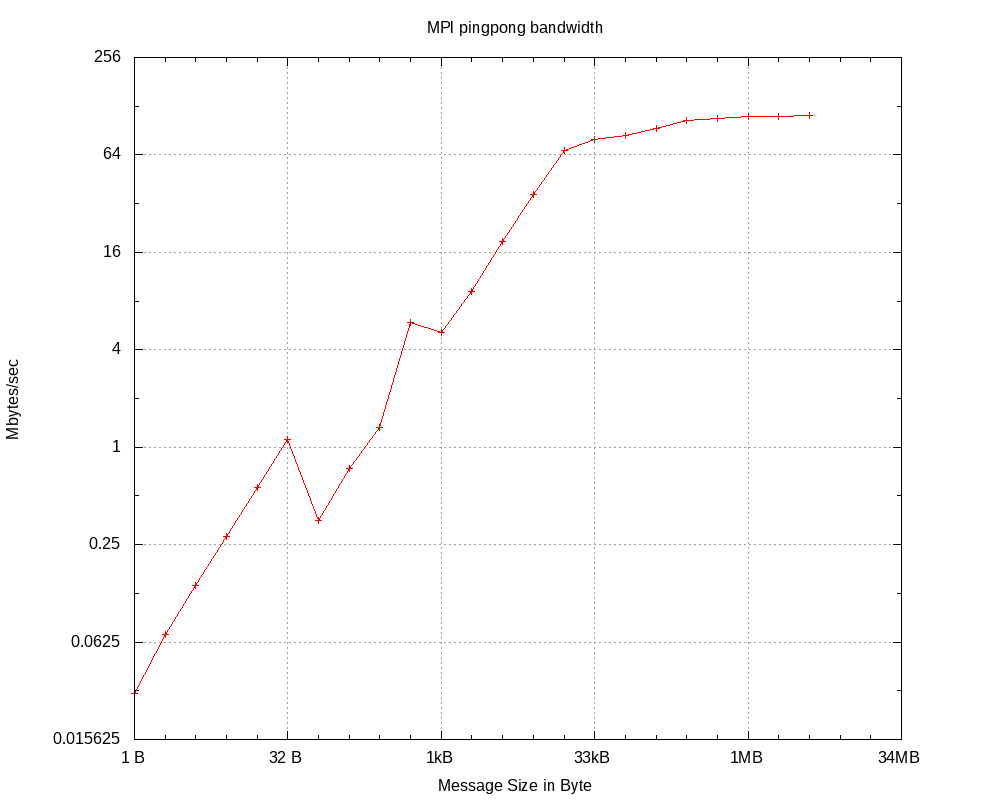
\includegraphics[scale=0.6]{../mpi_benchmark/pingpong_bandwidth.png} 
\newline
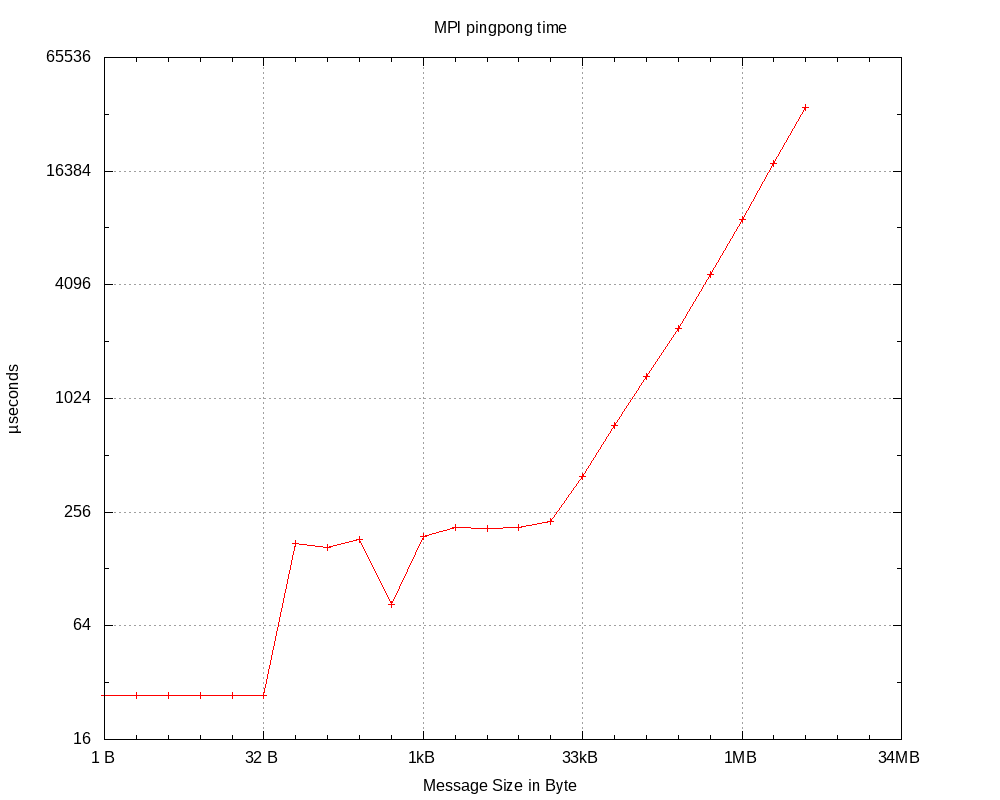
\includegraphics[scale=0.6]{../mpi_benchmark/pingpong_time.png}
\subsection{Gruppenkommunikationen}
Benchmark starten:
\begin{lstlisting}[style=Bash]
$ /shared/tools/openmpi/1.8.4/bin/mpirun -n 6 -hostfile /shared/mpi \
    _hosts ./IMB-MPI1 barrier allreduce alltoall \
	-off_cache -2048,64 -npmin 6
\end{lstlisting}
Ausgabe:
\lstinputlisting[style=BASH]{../mpi_benchmark/mpi_barrier_allreduce_alltoall}
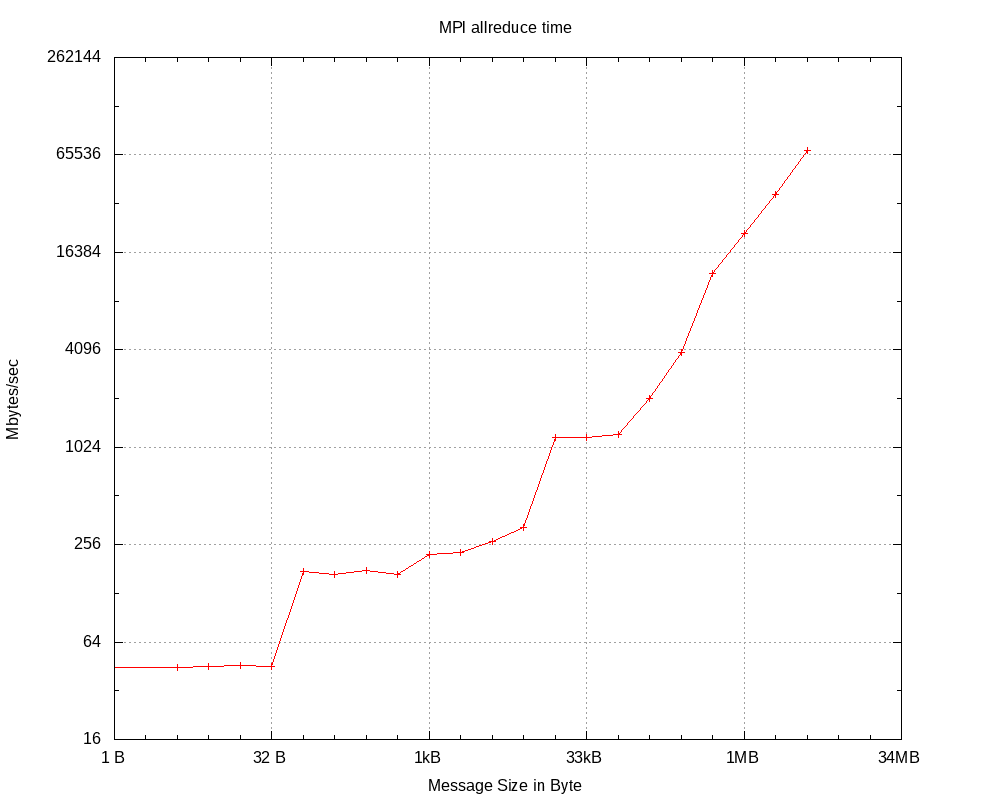
\includegraphics[scale=0.6]{../mpi_benchmark/allreduce_time.png}
\newline
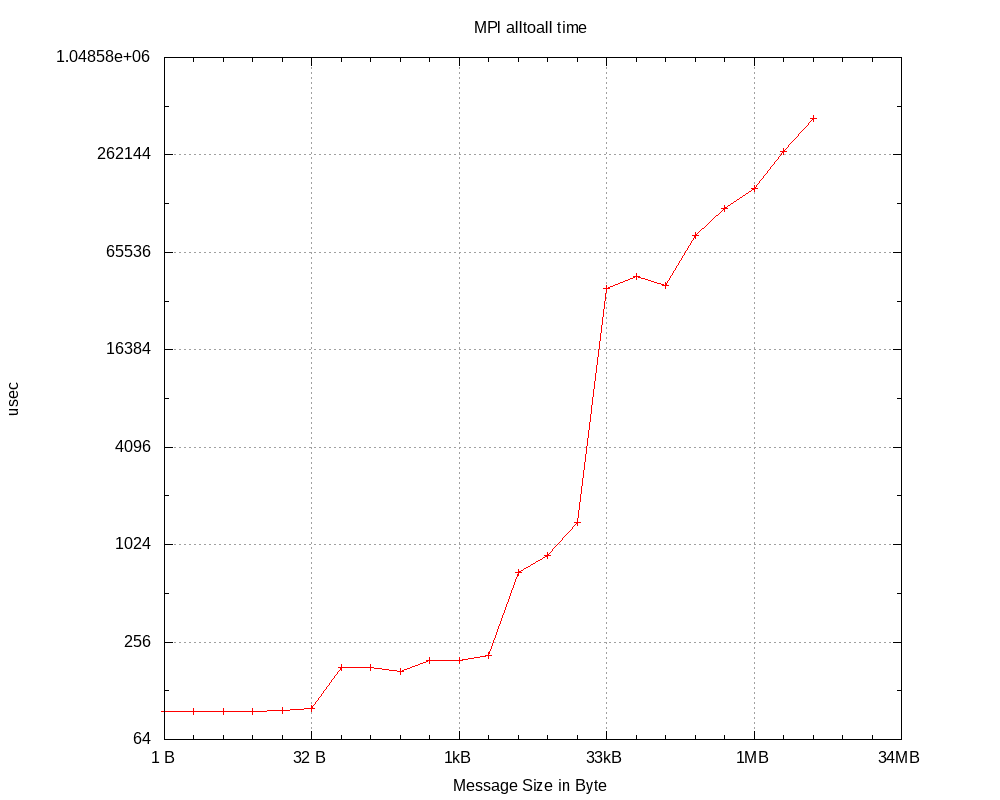
\includegraphics[scale=0.6]{../mpi_benchmark/alltoall_time.png}
\section{iozone}
\begin{lstlisting}[style=Bash]
/etc/apt/sources.list non-free
# apt-get update
# apt-get install iozone3
iozone -a -i 0 -g 512M -F /shared/iotmp > out.txt
$ ./GenGraph out.text
\end{lstlisting}
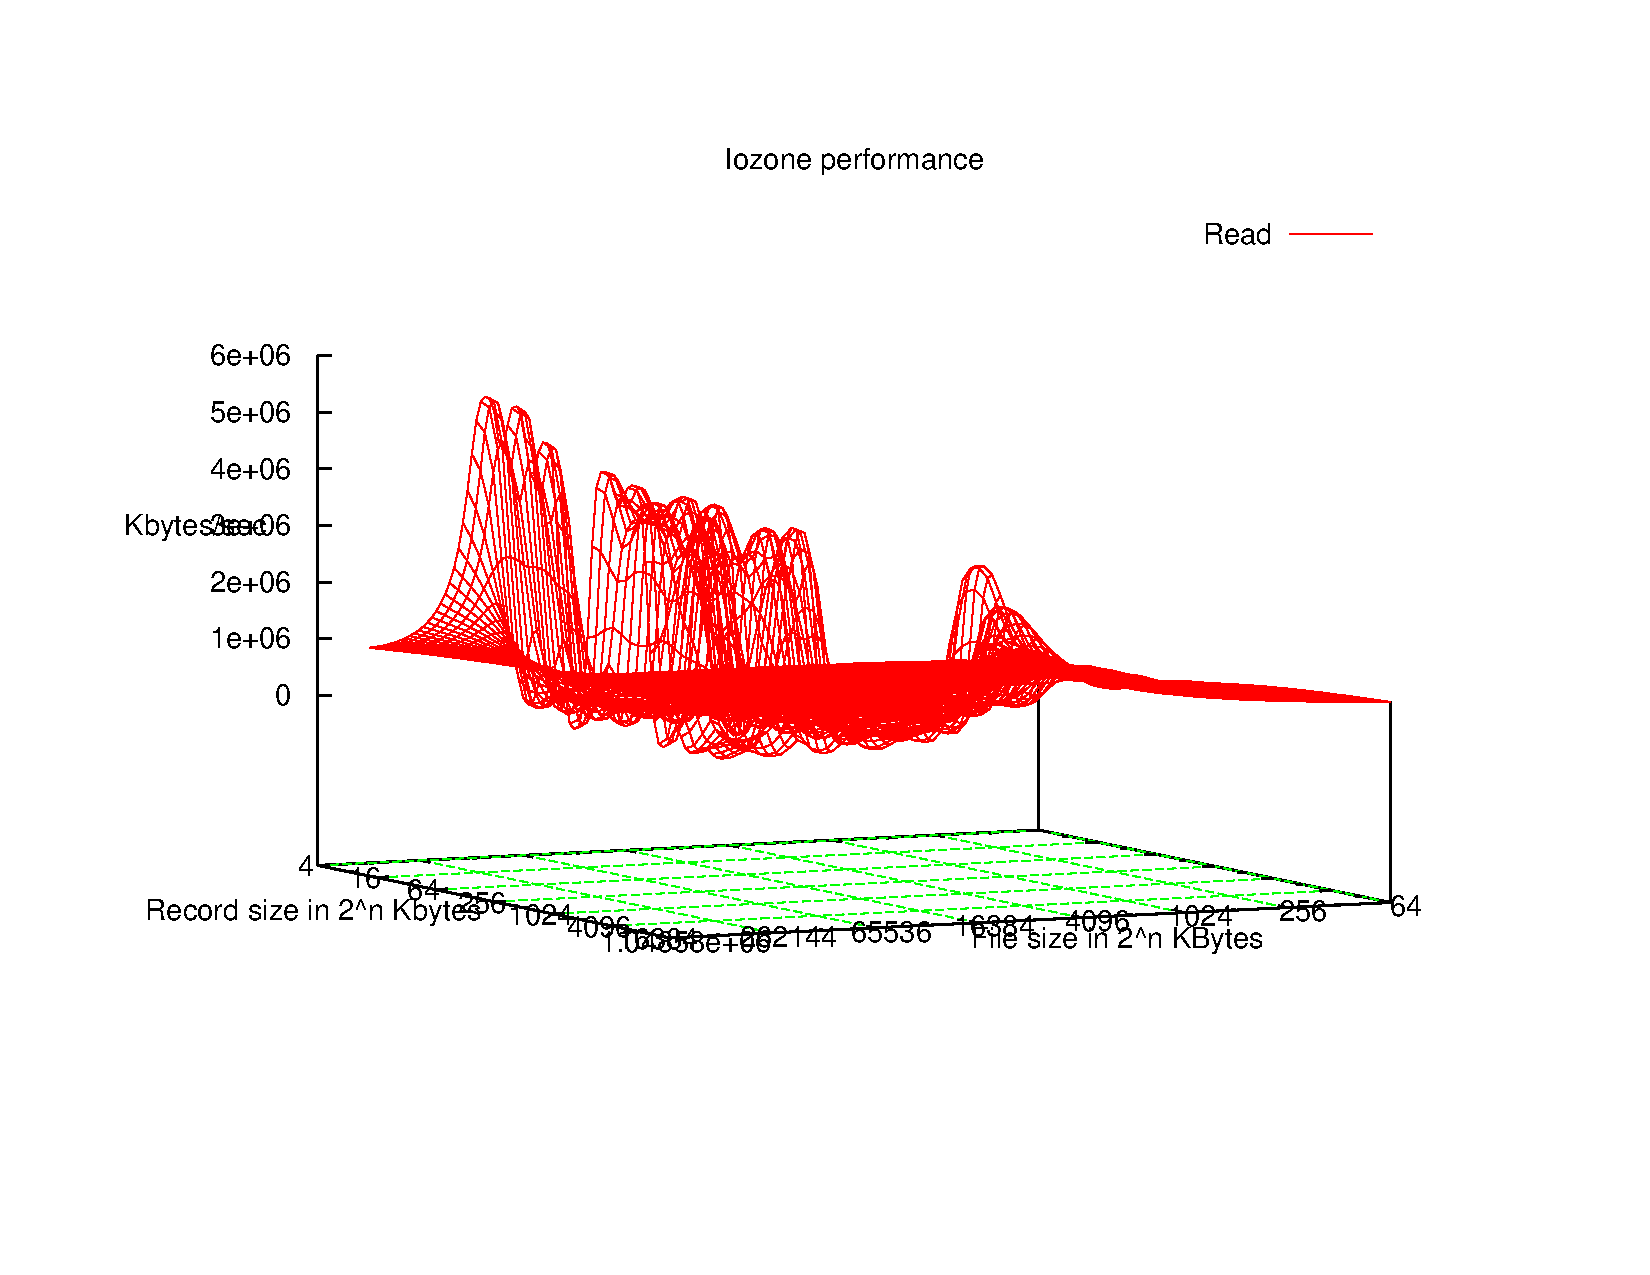
\includegraphics[scale=0.7]{read.pdf}
